\documentclass[conference]{IEEEtran}
\usepackage{amsmath}
\usepackage{graphicx}
\usepackage{listings}
\usepackage{xcolor}
\usepackage{hyperref}
\usepackage{algorithm}
\usepackage{algorithmic}
\usepackage{mathtools}
\usepackage{enumitem}
\usepackage{booktabs}
\usepackage{titlesec}
\usepackage{setspace}
\usepackage{tikz}
\usepackage{pgfplots}

% Configure column spacing
\setlength{\columnsep}{4em}

% Configure title format
\titleformat{\section}
  {\normalfont\large\bfseries}
  {\arabic{section}}
  {1em}
  {}
\titlespacing*{\section}{0pt}{1ex plus 0.5ex minus .2ex}{1ex plus .2ex}

\titleformat{\subsection}
  {\normalfont\bfseries}
  {\arabic{section}.\arabic{subsection}}
  {1em}
  {}
\titlespacing*{\subsection}{0pt}{0.75ex plus 0.5ex minus .2ex}{0.75ex plus .2ex}

% Configure listings
\lstset{
    basicstyle=\small\ttfamily,
    breaklines=true,
    frame=single,
    xleftmargin=1em,
    xrightmargin=1em
}

% Configure itemize and enumerate
\setlist{leftmargin=*}
\setlist[itemize]{label=$\bullet$}
\setlist[enumerate]{label=\arabic*.}

% Custom title command
\renewcommand{\maketitle}{%
  \begin{center}
    {\bfseries\large CS190I: Generative AI, Spring 2025\\
    Programming Assignment 2\\
    \normalsize Joe Lee\\
    \today}
  \end{center}
}

\begin{document}

\maketitle

\section{Model and Dataset Selection}
I implemented fine-tuning experiments using the T5-small model \cite{raffel2020exploring} for headline generation. The model was fine-tuned on the Gigaword 10k dataset \cite{gigaword}, which consists of news articles and their corresponding headlines. The task involves generating concise headlines from full news articles, making it an ideal candidate for testing different fine-tuning approaches.

\section{Implementation Details}

\subsection{Fine-tuning Approaches}
I implemented three distinct fine-tuning strategies:
\begin{enumerate}
    \item Full fine-tuning: Updates all model parameters
    \item Adapter fine-tuning: Adds trainable adapter layers
    \item LoRA fine-tuning: Implements low-rank updates with varying ranks
\end{enumerate}

\begin{table}[h]
\centering
\small
\setlength{\tabcolsep}{4pt}
\begin{tabular}{lrrrr}
\toprule
Method & BLEU & ROUGE-1 & ROUGE-2 & ROUGE-L \\
\midrule
Base Model & 4.85 & 0.30 & 0.10 & 0.27 \\
Full Fine-tuning & 18.75 & 0.44 & 0.22 & 0.42 \\
Adapter & 5.02 & 0.30 & 0.10 & 0.27 \\
LoRA (r=4) & 13.43 & 0.39 & 0.17 & 0.37 \\
LoRA (r=8) & 12.97 & 0.38 & 0.17 & 0.36 \\
LoRA (r=16) & 12.48 & 0.37 & 0.16 & 0.35 \\
\bottomrule
\end{tabular}
\caption{Performance metrics across different fine-tuning methods.}
\label{tab:performance}
\end{table}

\begin{figure}[h]
\centering
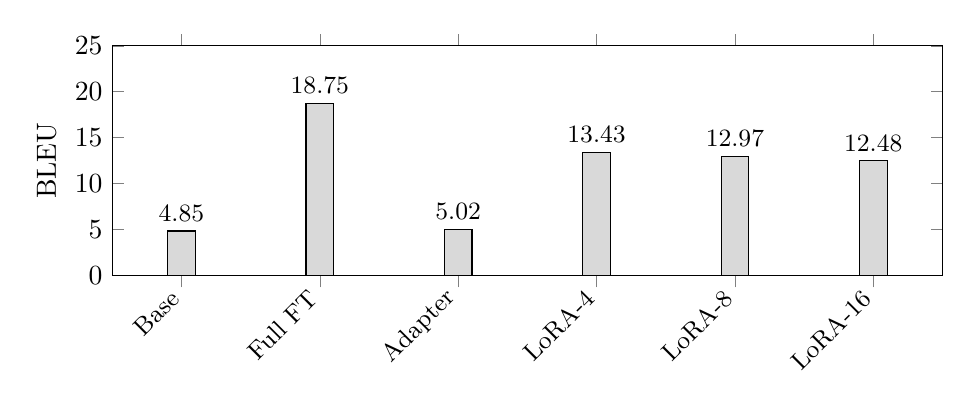
\begin{tikzpicture}
\begin{axis}[
    width=\columnwidth,
    height=4.5cm,
    ybar,
    bar width=10pt,
    ylabel={BLEU},
    symbolic x coords={Base, Full FT, Adapter, LoRA-4, LoRA-8, LoRA-16},
    xtick=data,
    xticklabel style={rotate=45, anchor=east, font=\small},
    ymin=0,
    ymax=25,
    ytick={0,5,10,15,20,25},
    nodes near coords,
    nodes near coords align={vertical},
    nodes near coords style={font=\small},
    ]
\addplot[fill=gray!30] coordinates {
    (Base, 4.85)
    (Full FT, 18.75)
    (Adapter, 5.02)
    (LoRA-4, 13.43)
    (LoRA-8, 12.97)
    (LoRA-16, 12.48)
};
\end{axis}
\end{tikzpicture}
\caption{BLEU scores across different fine-tuning methods.}
\label{fig:bleu_scores}
\end{figure}

\subsection{Training Configuration}
Training was performed on an NVIDIA RTX 3090 24GB GPU with the following parameters:
\begin{itemize}
    \item Batch size: 32
    \item Learning rate: 3e-4
    \item Optimizer: AdamW
    \item Evaluation metrics: BLEU, ROUGE-1, ROUGE-2, ROUGE-L
\end{itemize}

\begin{table}[h]
\centering
\small
\setlength{\tabcolsep}{4pt}
\setlength{\belowcaptionskip}{-10pt}
\begin{tabular}{lr}
\toprule
Method & Time (s) \\
\midrule
Full Fine-tuning & 549 \\
Adapter & 432 \\
LoRA (r=4) & 426 \\
LoRA (r=8) & 427 \\
LoRA (r=16) & 462 \\
\bottomrule
\end{tabular}
\end{table}

\section{Program Usage}
The implementation includes three main components:
\begin{itemize}
    \item \texttt{train.py}: Training script with configurable parameters for model type, output directory, batch size, epochs, and learning rate
    \item \texttt{eval.py}: Evaluation script for computing metrics and saving results
    \item \texttt{inference.py}: Script for generating headlines from input text using the fine-tuned models
\end{itemize}

Please check \texttt{README.md} for more details on how to run the program.

\section{Analysis and Discussion}

\subsection{Accuracy Improvements}
The results demonstrate significant improvements over the base model:
\begin{itemize}
    \item Full fine-tuning achieved the best performance (BLEU: 18.75)
    \item LoRA fine-tuning provided a good balance between performance and efficiency
    \item Adapter fine-tuning showed minimal improvement over the base model
\end{itemize}

\subsection{Impact of LoRA Rank}
Analysis of different LoRA ranks reveals:
\begin{itemize}
    \item Lower ranks (r=4) achieved better performance
    \item Higher ranks led to slightly worse results
    \item Training time increased with rank size
\end{itemize}

\section{Lessons Learned}
\begin{itemize}
    \item Full fine-tuning provides the best accuracy but requires more computational resources
    \item LoRA offers an excellent trade-off between performance and efficiency
    \item Adapter fine-tuning may require more careful architecture design for this specific task
    \item Lower LoRA ranks can be more effective than higher ones, suggesting that the task doesn't require complex parameter updates
\end{itemize}

\begin{thebibliography}{9}
\bibitem{raffel2020exploring}
C. Raffel, N. Shazeer, A. Roberts, K. Lee, S. Narang, M. Matena, Y. Zhou, W. Li, and P. J. Liu,
``Exploring the Limits of Transfer Learning with a Unified Text-to-Text Transformer,''
\textit{Journal of Machine Learning Research}, vol. 21, no. 140, pp. 1-67, 2020.

\bibitem{gigaword}
A. Mafzal,
``Gigaword 10k Finetuning Dataset,''
Hugging Face Datasets, 2023.
[Online]. Available: \url{https://huggingface.co/datasets/anumafzal94/gigaword_10k_finetuning}
\end{thebibliography}

\end{document} 